\documentclass{beamer}

\usefonttheme{serif}
\beamertemplatenavigationsymbolsempty
\setbeamertemplate{footline}[frame number]
\usecolortheme[named=violet]{structure}

\usepackage{geometry}
\usepackage{amssymb, amsmath, amsthm}
\usepackage{enumitem}
\usepackage{pgf,tikz}
\usepackage{listings}
\usepackage{algorithm}
\usepackage{algpseudocode}
\usepackage{svg}
\usepackage[dvipsnames]{xcolor}
\usepackage{tabularx}

\lstset{
    commentstyle=\color{SeaGreen},
    keywordstyle=\color{magenta},
    numberstyle=\tiny\color{Gray},
    stringstyle=\color{codepurple},
    basicstyle=\ttfamily\footnotesize,
    breaklines=true,                 
    captionpos=b,                    
    keepspaces=true,                 
    numbers=left,                    
    numbersep=5pt,                  
    showspaces=false,                
    showstringspaces=false,
    showtabs=false,                  
    tabsize=4,
}
\lstloadlanguages{C}

\renewcommand{\algorithmicrequire}{\textbf{Input:}}
\renewcommand{\algorithmicensure}{\textbf{Output:}}

\newcommand{\Q}{\mathbb{Q}}
\newcommand{\Z}{\mathbb{Z}}
\newcommand{\N}{\mathbb{N}}
\newcommand{\angles}[1]{\langle #1 \rangle}
\newcommand{\dd}{\mathop{}\!d}
\newcommand{\its}[1]{\textcolor{violet}{\emph{#1}}}

\newtheorem{proposition}{Proposition}

\setbeamertemplate{theorems}[normal font]
\newcommand{\labelitemi}{$\color{violet}{\blacktriangleright}$} 

\title{COSC3500 Project}
\subtitle{Milestone 2 (Parallel)}
\author{Mitchell Holt}
\date{November 2024}

\begin{document}

\titlegraphic{
\includegraphics[width=.37\textwidth]{thinker.jpg}}

\begin{frame}
    \maketitle
\end{frame}

\begin{frame}
    \frametitle{FFT Polynomial Multiplication}

    Let $F$ be a field and $f,g \in F[x]$. \pause \vfill

    \begin{enumerate}[label=(\roman*)]
        \item The classical multiplication algorithm is $O(n^2)$. \pause
            \medbreak

        \item Write $f = f_0 + f_1x + \cdots + f_{n - 1} x^{n - 1}$ and consider
            $\begin{bmatrix} \omega^0 & \omega^1 & \cdots & \omega^{n - 1}
            \end{bmatrix}$, where $\omega \in F$ is a \its{primitive $n$-th root
            of unity}. \pause \medbreak

        \item The FFT to computes the \its{multi-point evaluation map}
            $$
                \begin{bmatrix} f_0 & f_1 & \cdots & f_{n - 1} \end{bmatrix}
                \quad \mapsto \quad \begin{bmatrix}
                    f(\omega^0) & f(\omega^1) & \cdots & f(\omega^{n - 1})
                \end{bmatrix}
            $$
            and the \its{interpolation map}
            $$
                \begin{bmatrix}
                    f(\omega^0) & f(\omega^1) & \cdots & f(\omega^{n - 1})
                \end{bmatrix}
                \quad \mapsto \quad
                \begin{bmatrix} f_0 & f_1 & \cdots & f_{n - 1} \end{bmatrix}
            $$
            in $O(n\log n)$ time.
    \end{enumerate}
\end{frame}

\begin{frame}
    \frametitle{FFT Polynomial Multiplication}

    \begin{algorithmic}
        \Require $n = 2^k$, $f,g \in F[x]$ with degree less than $n/2$,
        $\omega \in F$ a primitive $n$-th root of unity
        \Ensure $fg$
        \pause \vfill

        \State $A \gets$ FFT evaluation of $f$ at
            $\begin{bmatrix} \omega^0 & \cdots & \omega^{n - 1} \end{bmatrix}$
        \State $B \gets$ FFT evaluation of $g$ at
            $\begin{bmatrix} \omega^0 & \cdots & \omega^{n - 1} \end{bmatrix}$
        \pause \vfill

        \For{$i = 0,1,\dots,n - 1$} \State $C_i \gets A_i \cdot B_i$ \EndFor
        \pause \vfill

        \State $h \gets$ FFT interpolation from $C$.
        \State \Return $h$
    \end{algorithmic}
\end{frame}

\begin{frame}
    \frametitle{A Tale of Two Algorithms}

    We can make the FFT in-place at the cost of introducing permutations. There
    are two \its{dual} algorithms:

    \begin{figure}[h]
        \centering
        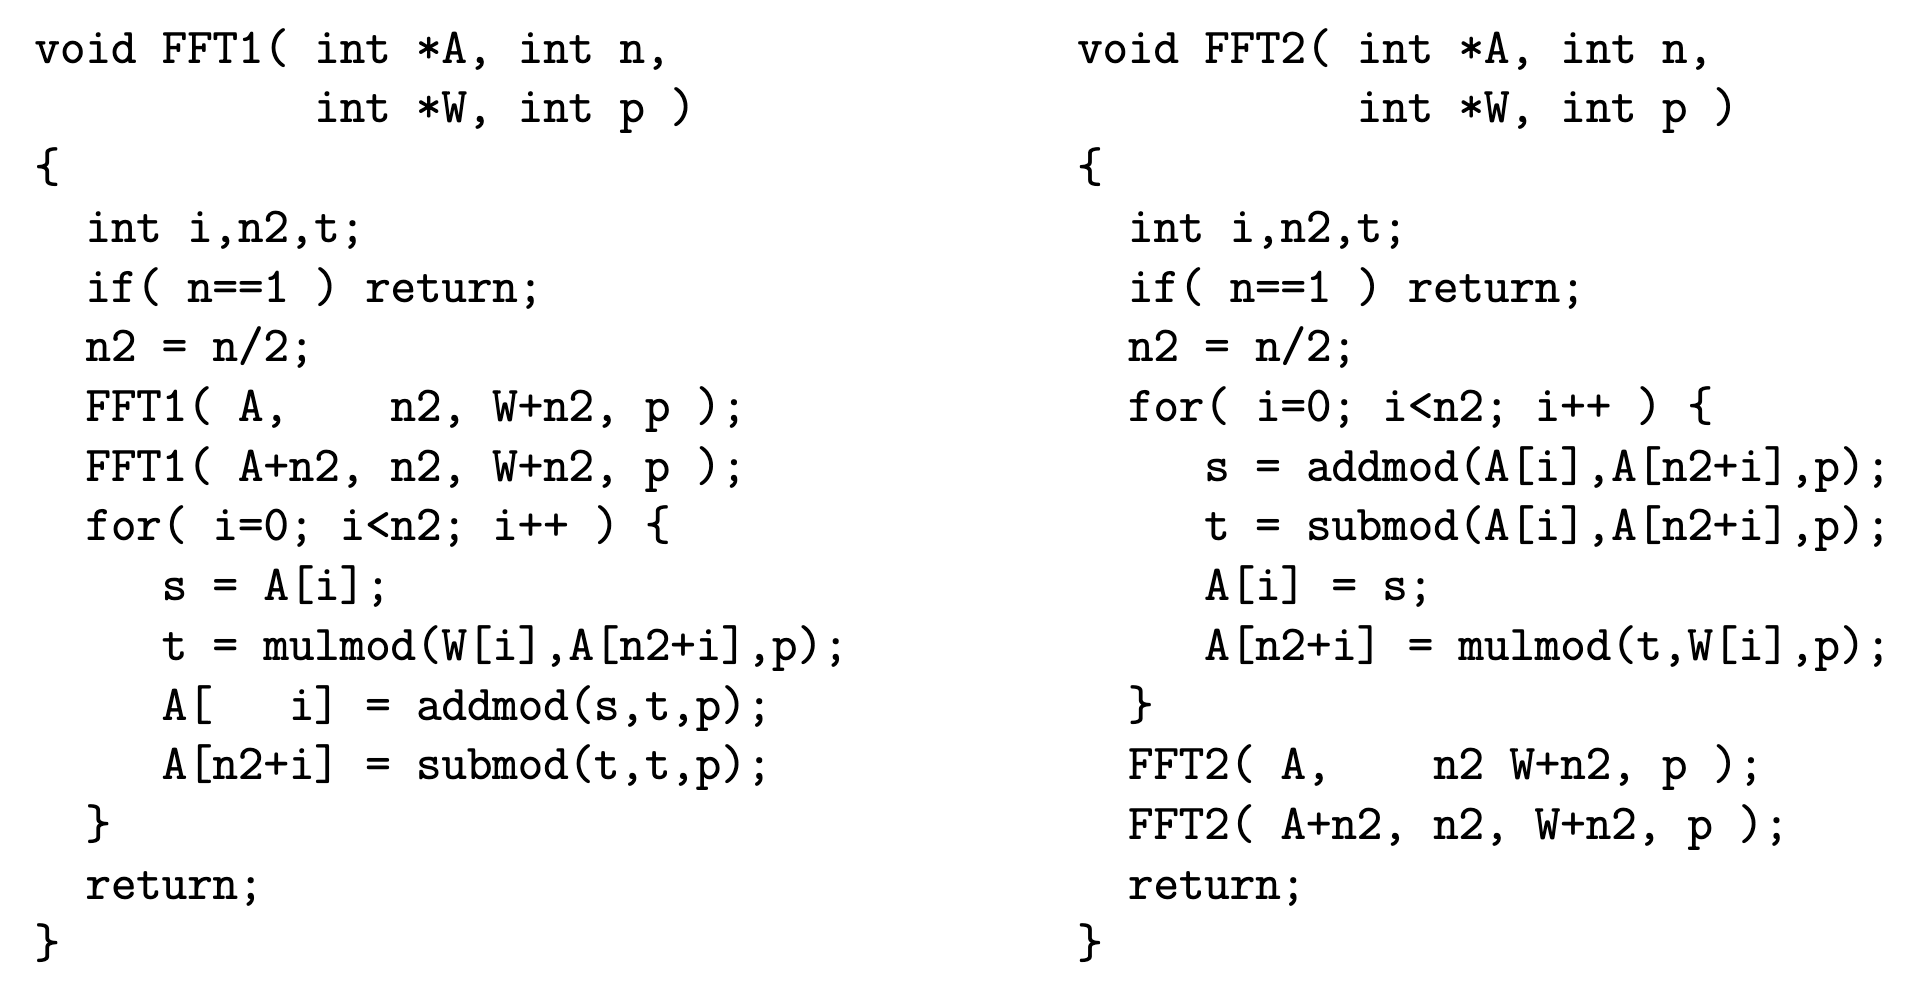
\includegraphics[width=0.9\textwidth]{monagan.png}
        \caption{Monagan's example code \cite{monagan}}
    \end{figure}
\end{frame}

\begin{frame}
    \frametitle{Serial Code Performance}

    For reference, the Maple computer algebra system averages 13ms per
    multiplication of size $2^{15}$.

    \begin{figure}
        \centering
        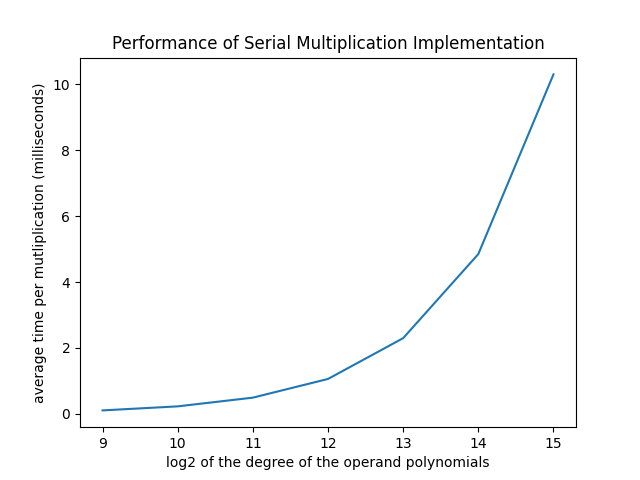
\includegraphics[width=0.8\textwidth]{initial.png}
    \end{figure}
\end{frame}

\begin{frame}
    \frametitle{Serial Code Performance}

    Modular arithmetic is (unsurprisingly) a significant bottleneck.

    \vfill

    \begin{table}
        \centering
        \begin{tabularx}{0.7\textwidth}{ 
                | >{\centering\arraybackslash}X | >{\centering\arraybackslash}X | >{\centering\arraybackslash}X |
            }
            \hline
            \textbf{Function}       & \textbf{Runtime} \\
            \hline
            \lstinline{addmod}         & 22.81\% \\
            \lstinline{mulmod}         & 21.11\% \\
            \lstinline{submod}         & 11.73\% \\
            \lstinline{triple\_mulmod} & 2.98\% \\
            \hline
            \textbf{Total}          & \textbf{68.63\%} \\
            \hline
        \end{tabularx}
        \caption{selection from \lstinline{gprof} flat profile}
    \end{table}
\end{frame}

\begin{frame}
    \frametitle{SIMD Modular Arithmetic}

    \begin{enumerate}[label=(\roman*)]
        \item Need to compute $x + y \mod p$ and $x - y \mod p$. \pause
            \medbreak

        \item There are no SIMD instructions for computing remainders.
            \begin{figure}
                \centering
                
\includegraphics[width=0.5\textwidth]{this_could_be_us.png}
                \caption{this could be us}
            \end{figure}

            \pause \medbreak

        \item I implemented the addition algorithm from \cite{simd}, but wrote
            my own subtraction and multiplication.
    \end{enumerate}
\end{frame}

% \begin{frame}
%     \frametitle{SIMD Modular Subtraction}
%     % Explain the subtraction algorithm 
% 
%     % Why 128-bit packed integers? Tried getting 8 integers through at a time in
%     % the serial optimisation (that is, unrolling to 8) and it was much slower.
%     % This is probably because we are trying to work with 3 arrays, so stuff gets
%     % evicted from L1. Therefore we stuck with 4 integers at a time here.
% 
% \end{frame}

\begin{frame}
    \frametitle{SIMD Modular Multiplication}

    \begin{enumerate}[label=(\roman*)]
        \item The product of any two integers we multiply may be too large to
            fit in a 32-bit integer, so we need to produce intermediate 64-bit
            integers. \pause \medbreak

        \item Need to use twice as many vector operations! \pause \medbreak

        \item As there is no SIMD remainder instruction, we recover
            $a \cdot b \mod 2^{16} + 1$ as follows:
            $$
                a \cdot b = q \cdot 2^{16} + r = q \cdot (2^{16} + 1) + r - q
            $$
            \pause Therefore $a \cdot b \mod 2^{16} + 1 = r - q$.
    \end{enumerate}
\end{frame}

\begin{frame}
    \frametitle{SIMD Modular Multiplication}

    \begin{enumerate}[label=(\roman*)]
        \item Sometimes we need to compute $a \cdot b \cdot c \mod p$.
            \pause \medbreak

        \item Idea: only perform a single mod operation. \pause \medbreak

        \item This requires 64-bit multipliction, but the only SIMD intrinsics
            that do this require AVX-512 \pause \medbreak

        \item \lstinline{\_mm\_mullo\_epi64} and friends all have
            \its{15 cycle latency}.
    \end{enumerate}
\end{frame}

\begin{frame}
    \frametitle{SIMD in the FFT base cases}

    Inlined and unrolled the 3 smallest recursive calls to \lstinline{fft1} and
    \lstinline{fft2} ($n = 1,2,4$). 

    \begin{figure}[h]
        \centering
        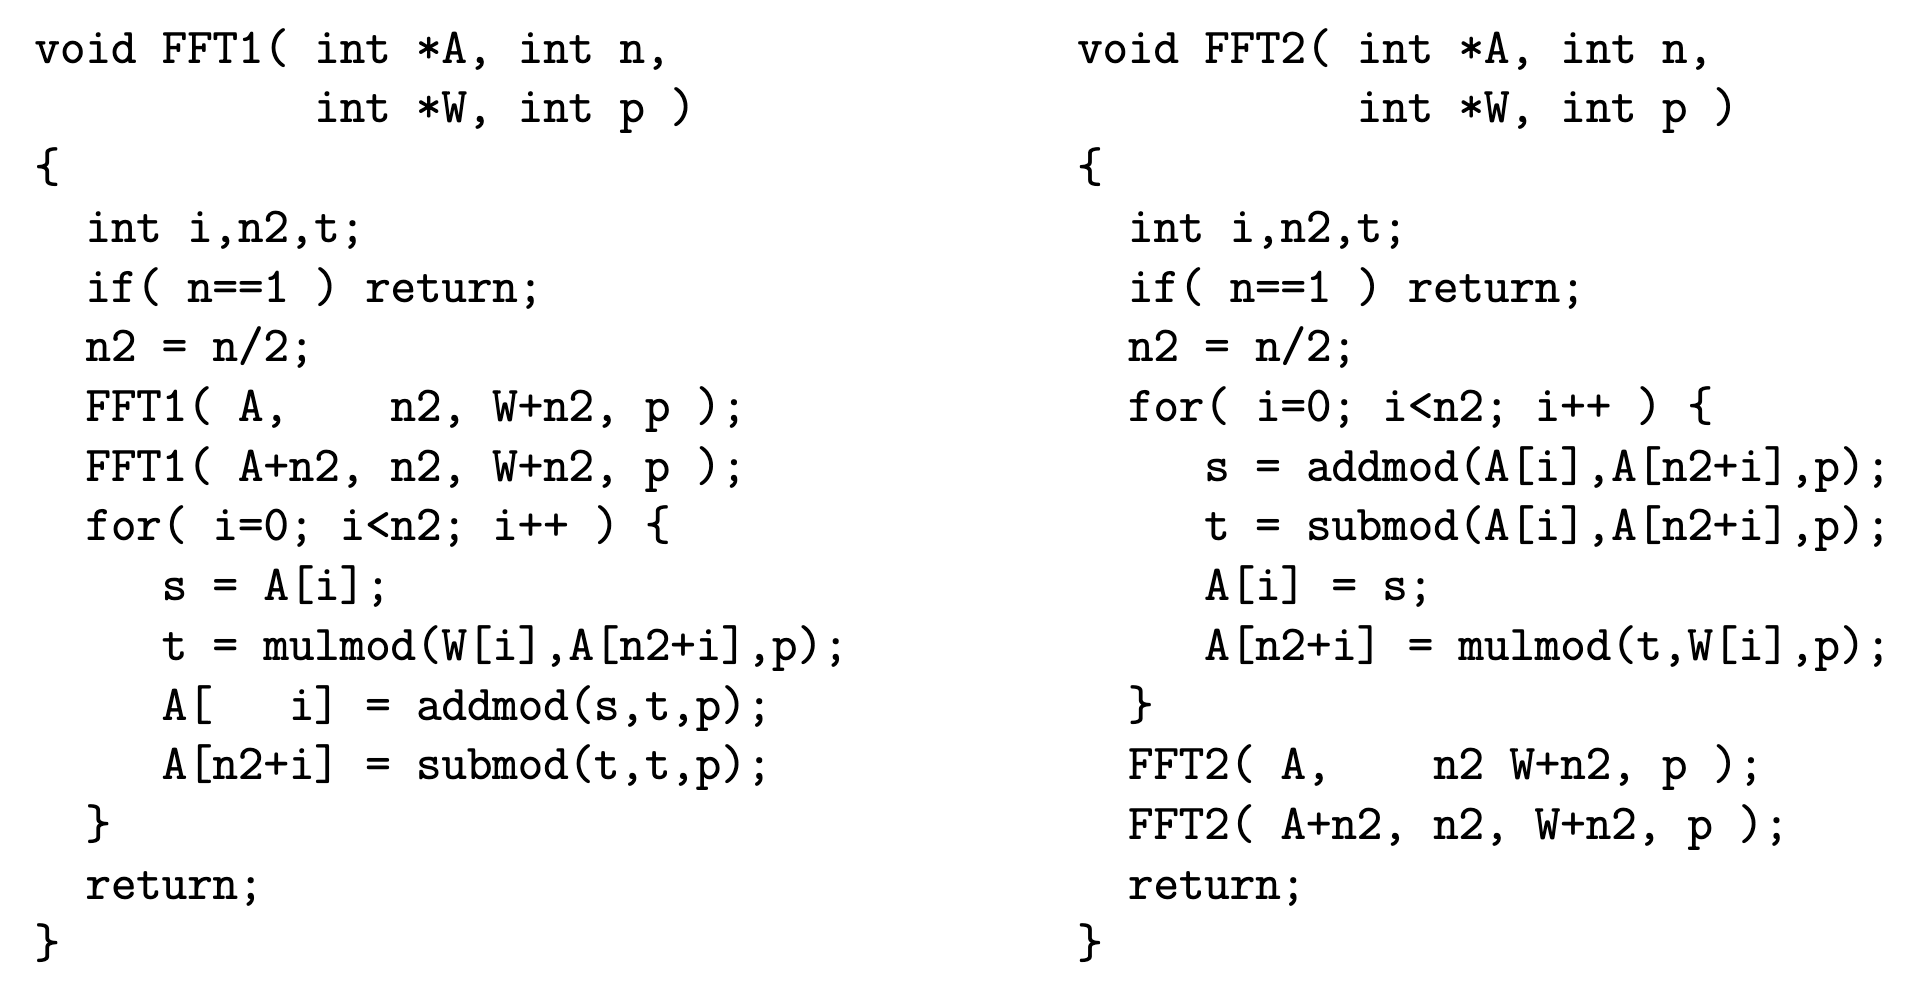
\includegraphics[width=0.9\textwidth]{monagan.png}
        \caption{Monagan's example code \cite{monagan}}
    \end{figure}

    \pause \vfill

    Vectorising this removes \its{all} scalar arithmetic in polynomial
    multiplication.
\end{frame}

\begin{frame}
    \frametitle{SIMD Code Performance}

    For reference, the Maple computer algebra system averages 13ms per
    multiplication of size $2^{15}$.

    \vfill

    \begin{figure}
        \centering
        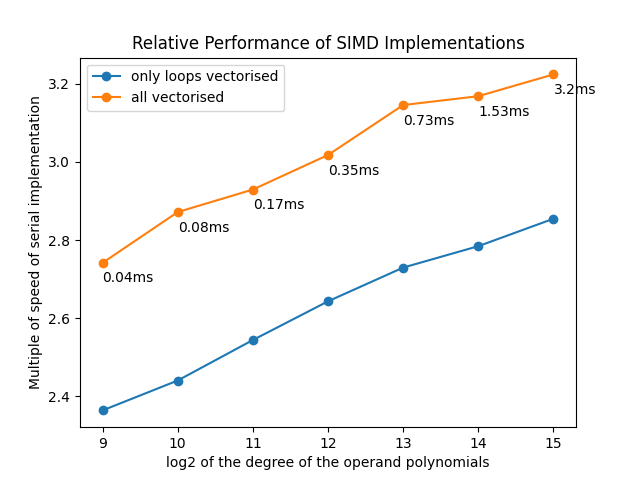
\includegraphics[width=0.7\textwidth]{avx_perf.png}
        \caption{performance of SIMD implementations}
    \end{figure}

\end{frame}

\begin{frame}
    \frametitle{OpenMP}

    \begin{enumerate}[label=(\roman*)]
        \item First, just ran loops in parallel. This was \its{significantly}
            slower. \pause
            \begin{itemize}
                \item Loops bodies are \its{very} fast \pause
                \item Cache/memory bandwidth problems when working with 3 arrays
                    at once.
            \end{itemize}
            \pause \medbreak

        \item Running recursive calls in parallel. \pause
            \begin{itemize}
                \item Each recursive call creates two new recursive calls. In
                    total, as many as $2 \cdot 16 - 1 = 31$ calls. \pause
                \item  Only 8 physical cores. \pause
                \item Only run the topmost $k$ calls in parallel
                \item Stopping at depth $2$ was fastest.
            \end{itemize}

            \vfill

            \begin{center}
                \includesvg[width=0.6\textwidth]{rec_depth.svg}
            \end{center}
    \end{enumerate}

\end{frame}

\begin{frame}
    \frametitle{OpenMP Code Performance}

    For reference, the Maple computer algebra system averages 13ms per
    multiplication of size $2^{15}$.

    \vfill

    \begin{figure}
        \centering
        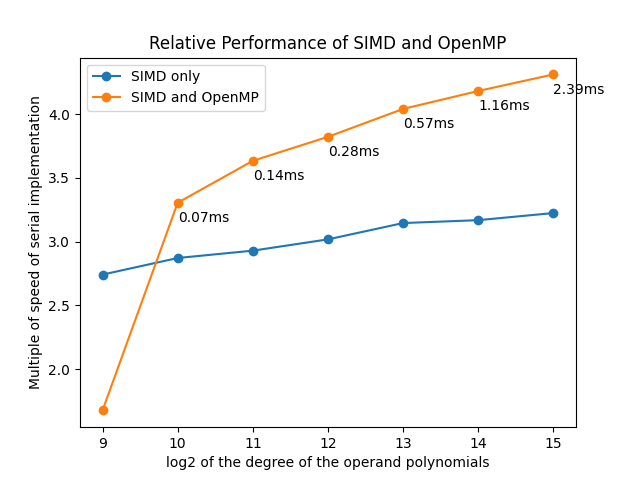
\includegraphics[width=0.7\textwidth]{omp_perf.png}
        \caption{performance of OpenMP implementation}
    \end{figure}

\end{frame}

\begin{frame}
    \frametitle{Reflection and Conclusion}

    \begin{enumerate}[label=(\roman*)]
        \item My problem has a maximum size (polynomial operands of degree
            $2^{15}$) \pause \medbreak

        \item No vector mod instruction meant I had to write some funky code.
            \pause \medbreak

        \item SIMD is \its{fast}. \pause \medbreak

        \item I'm more than 5 times faster than Maple\footnote<4->{
                Admittedly, I don't have to decide what kernel code to use at
                runtime, and I do cheat a little bit.
            }. \pause \medbreak

        \item \its{Extension:} Stop cheating. Implement a modular multiplication
            algorithm that works for \its{any} prime.
    \end{enumerate}
\end{frame}

\begin{frame}
    \frametitle{References}

    \bibliographystyle{alpha}
    \bibliography{bibliography}
\end{frame}

\end{document}
